% Figure from MATH 591 notes, section 70. Added, not from lecture (Lecture 25): left-invariant field on the ax+b group.
\begin{tikzpicture}[x=1cm, y=1.1cm]
\fill[black!3] (-3,0) rectangle (3.2,3);
\draw[black!50, dashed] (-3,0) -- (3.2,0) node[right, font=\scriptsize, text=black] {$a = 0$ (not in $G$)};
\draw[->, gray!70] (0,-0.15) -- (0,3.2) node[above, font=\scriptsize, text=black] {$a$};
\node[font=\scriptsize, gray] at (3.35,2.85) {$b$};
\draw[->, black!35] (-2.50,0.50) -- (-2.36,0.57);
\draw[->, black!35] (-2.50,1.00) -- (-2.22,1.14);
\draw[->, black!35] (-2.50,1.50) -- (-2.08,1.71);
\draw[->, black!35] (-2.50,2.00) -- (-1.94,2.28);
\draw[->, black!35] (-2.50,2.50) -- (-1.80,2.85);
\draw[->, black!35] (-1.50,0.50) -- (-1.36,0.57);
\draw[->, black!35] (-1.50,1.00) -- (-1.22,1.14);
\draw[->, black!35] (-1.50,1.50) -- (-1.08,1.71);
\draw[->, black!35] (-1.50,2.00) -- (-0.94,2.28);
\draw[->, black!35] (-1.50,2.50) -- (-0.80,2.85);
\draw[->, black!35] (-0.50,0.50) -- (-0.36,0.57);
\draw[->, black!35] (-0.50,1.00) -- (-0.22,1.14);
\draw[->, black!35] (-0.50,1.50) -- (-0.08,1.71);
\draw[->, black!35] (-0.50,2.00) -- (0.06,2.28);
\draw[->, black!35] (-0.50,2.50) -- (0.20,2.85);
\draw[->, black!35] (0.50,0.50) -- (0.64,0.57);
\draw[->, black!35] (0.50,1.00) -- (0.78,1.14);
\draw[->, black!35] (0.50,1.50) -- (0.92,1.71);
\draw[->, black!35] (0.50,2.00) -- (1.06,2.28);
\draw[->, black!35] (0.50,2.50) -- (1.20,2.85);
\draw[->, black!35] (1.50,0.50) -- (1.64,0.57);
\draw[->, black!35] (1.50,1.00) -- (1.78,1.14);
\draw[->, black!35] (1.50,1.50) -- (1.92,1.71);
\draw[->, black!35] (1.50,2.00) -- (2.06,2.28);
\draw[->, black!35] (1.50,2.50) -- (2.20,2.85);
\draw[->, black!35] (2.50,0.50) -- (2.64,0.57);
\draw[->, black!35] (2.50,1.00) -- (2.78,1.14);
\draw[->, black!35] (2.50,1.50) -- (2.92,1.71);
\draw[->, black!35] (2.50,2.00) -- (3.06,2.28);
\draw[->, black!35] (2.50,2.50) -- (3.20,2.85);
\draw[blue!70!black, very thick, ->] plot coordinates {(-1.940,0.030) (-1.839,0.080) (-1.739,0.131) (-1.638,0.181) (-1.537,0.231) (-1.437,0.282) (-1.336,0.332) (-1.235,0.382) (-1.135,0.433) (-1.034,0.483) (-0.933,0.533) (-0.833,0.584) (-0.732,0.634) (-0.631,0.684) (-0.531,0.735) (-0.430,0.785) (-0.329,0.835) (-0.228,0.886) (-0.128,0.936) (-0.027,0.986) (0.074,1.037) (0.174,1.087) (0.275,1.137) (0.376,1.188) (0.476,1.238) (0.577,1.288) (0.678,1.339) (0.778,1.389) (0.879,1.439) (0.980,1.490) (1.080,1.540) (1.181,1.591) (1.282,1.641) (1.382,1.691) (1.483,1.742) (1.584,1.792) (1.684,1.842) (1.785,1.893) (1.886,1.943) (1.986,1.993) (2.087,2.044) (2.188,2.094) (2.288,2.144) (2.389,2.195) (2.490,2.245) (2.591,2.295) (2.691,2.346) (2.792,2.396) (2.893,2.446) (2.993,2.497) (3.094,2.547) (3.195,2.597)};
\fill[blue!70!black] (0.0,1.0) circle (1.8pt) node[above left, font=\scriptsize] {$e = (1, 0)$};
\draw[red!70!black, very thick, ->] plot coordinates {(0.560,0.030) (0.661,0.080) (0.761,0.131) (0.862,0.181) (0.963,0.231) (1.063,0.282) (1.164,0.332) (1.265,0.382) (1.365,0.433) (1.466,0.483) (1.567,0.533) (1.667,0.584) (1.768,0.634) (1.869,0.684) (1.969,0.735) (2.070,0.785) (2.171,0.835) (2.272,0.886) (2.372,0.936) (2.473,0.986) (2.574,1.037) (2.674,1.087) (2.775,1.137) (2.876,1.188) (2.976,1.238) (3.077,1.288) (3.178,1.339)};
\fill[red!70!black] (1.5,0.5) circle (1.8pt) node[below right, font=\scriptsize] {$g = (\tfrac12, \tfrac32)$};
\fill[blue!70!black] (1.297,1.649) circle (1.5pt) node[above left, font=\scriptsize] {$\varphi^e(1)$};
\fill[red!70!black] (2.149,0.824) circle (1.5pt) node[below right, font=\scriptsize] {$g\,\varphi^e(1)$};
\draw[->, black!60, dotted, thick] (1.217,1.679) to[bend right=25] node[above, font=\scriptsize] {$L_g$} (2.249,0.854);
\end{tikzpicture}
